\documentclass[11pt,a4paper]{article}
\usepackage[utf8]{inputenc}
\usepackage[T1]{fontenc}
\usepackage{textcomp}
\usepackage{lmodern}
\usepackage[margin=1in]{geometry}
\usepackage{amsmath,amssymb}
\usepackage{booktabs}
\usepackage{tabularx}
\usepackage{threeparttable}
\usepackage{graphicx}
\usepackage{float}
\usepackage{xcolor}
\usepackage{setspace}
\usepackage[authoryear,round]{natbib}
\usepackage[colorlinks=true,linkcolor=blue!60!black,citecolor=blue!60!black,urlcolor=blue!60!black]{hyperref}
\onehalfspacing

\newcommand{\gbp}{\textsterling}

\title{\textbf{Four Millennia of Information Friction: Real Communication Costs, Institutional Regimes, and Speed--Cost Trade-offs, 1895\,BC--2026\,AD}}
\author{Rolf Bastiaanssen}
\date{November 2026}

\begin{document}
\maketitle

\begin{abstract}
This paper constructs a four-millennium series of long-distance communication costs and transit latencies ($1895\,\text{BC}$--$2026\,\text{AD}$) across two primary inter-regional corridors---Antwerp--Venice and London--New York---anchored by Bronze Age, Roman, and Tang baselines. Normalizing nominal tariffs by contemporary local wages and separating delivery boundaries (door-to-door, terminal-to-terminal, and pure wire signaling) reveals two distinct phases prior to the twentieth century. Between $1395$ and $1855$, commercial postal networks reduced the real cost of sending a message by more than two orders of magnitude without altering physical transport speeds. In July $1866$, the transatlantic submarine telegraph inverted that relationship: transit latency fell from $292.8\,\text{hours}$ to $0.25\,\text{hours}$ terminal-to-terminal ($0.02\,\text{hours}$ of wire signaling), while real message costs rose $169$-fold ($3,381$-fold per word). Using a break-even quote-age model, we show that this tariff rationed early cable capacity to high-value commodity arbitrageurs until competitive cable entry ($1884$--$1888$) and optical multiplexing lowered unit costs. Finally, separating marginal wholesale backbone capacity ($1.30 \times 10^{-6}$ to $3.89 \times 10^{-9}\,\text{labor-hours}$ per message in $2026$) from retail broadband subscriptions resolves a persistent boundary bias in long-run price indices.
\end{abstract}

\noindent\textbf{JEL Classification:} N70, N71, N73, O33, L96.\\
\textbf{Keywords:} Communication costs, cliometrics, telegraphy, postal history, information frictions, market integration.

\section{Introduction}
\label{sec:introduction}

For nearly four millennia, the speed of long-distance communication was bounded by the physical pace of overland and maritime transport. Yet well before the electric telegraph broke that physical constraint, institutional reforms in European and transatlantic postal systems had already reduced the real cost of sending a message by more than two orders of magnitude. Between the late Roman Empire and the mid-nineteenth century, the cost of transmitting a standard commercial dispatch fell from nearly three hundred hours of unskilled labor to under two hours.

The opening of the permanent transatlantic submarine telegraph cable in July $1866$ temporarily reversed that secular decline. Transmission latency across the Atlantic fell from twelve days by steam packet to fifteen minutes terminal-to-terminal, and just over one minute of pure electrical signaling. At the same time, real message costs rose sharply. At the Anglo-American Telegraph Company's initial tariff of $\gbp 20$ for twenty words---and even after its November $1866$ reduction to $\gbp 10$---a single brief cablegram cost between $308$ and $615\,\text{hours}$ of skilled London labor, roughly $169$ times the price of a steam-packet letter and comparable in real terms to requisitioning an imperial carriage relay in late Roman Italy. High-speed messaging became broadly affordable only after competitive cable entry in the $1880\text{s}$ and twentieth-century coaxial and optical multiplexing.

This paper traces the joint evolution of communication costs and transit delays across two inter-regional corridors---Antwerp--Venice and London--New York---anchored by ancient and medieval baselines. Following \citet{Nordhaus1996} and \citet{Allen2001}, we express nominal tariffs in contemporary unskilled or building-craftsman \textit{labor-hours per standardized message} and \textit{labor-hours per 100 words} in the originating jurisdiction. Reporting unit-normalized costs alongside total message costs prevents shifts in message length from obscuring changes in the underlying price of information.

The remainder of the paper is organized as follows. Section~\ref{sec:methodology} sets out our num\'eraire conventions, operational transit boundaries, and three-tier source classification. Section~\ref{sec:pretelegraph} analyzes the pre-telegraphic decline in real communication costs from $1895\,\text{BC}$ to $1855\,\text{AD}$. Section~\ref{sec:telegraph} examines the $1866$ submarine cable shock, models the quote-age arbitrage threshold required to justify early telegraphic premiums, and traces price convergence through the $1880\text{s}$ cable wars and mid-twentieth-century coaxial telephony. Section~\ref{sec:optical} evaluates $2026$ optical networks and resolves the accounting boundary between wholesale backbone capacity and retail fixed broadband. Section~\ref{sec:conclusion} concludes.

\section{Measurement Framework, Operational Boundaries, and Source Hierarchy}
\label{sec:methodology}

Long-run comparisons of communication prices require strict controls across three dimensions: wage num\'eraires, message length, and delivery boundaries. First, to avoid exchange-rate distortions across pre-modern and modern monetary regimes, each nominal tariff is divided by the hourly wage of an unskilled laborer or urban building craftsman in the originating city during the same year (assuming a standard ten-hour workday prior to the twentieth century). Where statutory tariffs were levied per sheet or per half-ounce rather than per word, we evaluate both an empirically grounded commercial word count ($400\,\text{words}$ per sheet) and a conservative single-sheet statutory bound ($250\,\text{words}$).

Second, historical transit latencies are measured across three distinct operational boundaries:
\begin{enumerate}
    \item \textbf{Door-to-door (\texttt{D}):} End-to-end elapsed time from sender dispatch to recipient delivery, characteristic of caravans, couriers, and postal packets.
    \item \textbf{Terminal-to-terminal (\texttt{T}):} Elapsed time between central telegraph or telephone exchanges, including station queuing and local messenger delivery.
    \item \textbf{Wire-signaling-only (\texttt{W}):} Physical signal propagation and keying time across the transmission medium, excluding terminal handling.
\end{enumerate}
Because post-$1866$ records typically report terminal or wire speeds whereas pre-$1866$ postal records measure door-to-door transit, Table~\ref{tab:master_benchmarks} and Figure~\ref{fig:macro_spine} also include estimated door-to-door bounds for all post-$1866$ observations so that latency comparisons remain consistent across eras.

Third, to prevent heterogeneous historical evidence from being treated as observationally equivalent, every benchmark is scored independently for tariff pricing (\textit{Tariff Tier}) and payload or channel throughput (\textit{Capacity Tier}) across three tiers (detailed in Appendix~\ref{app:archival_ledger}): authenticated primary statutes, treaties, and tariff notices (\texttt{T1}); corroborated secondary historiography (\texttt{T2}); and parameterized institutional or engineering calibrations where open-access retail tariffs did not exist (\texttt{T3}). Where primary tablet transcriptions or local wage series remain incomplete, cells are left unpopulated rather than interpolated.

\section{Pre-Telegraphic Commercialization and Postal Integration, 1895\,BC--1855\,AD}
\label{sec:pretelegraph}

In antiquity and the early Middle Ages, rapid long-distance communication was organized primarily around state administration rather than open commercial carriage \citep{Innis1950}. Around $1895\,\text{BC}$, Old Assyrian merchants trading along the thousand-kilometer overland route between Assur and K\"ultepe in central Anatolia shipped clay correspondence inside donkey caravans that took roughly twenty-eight days ($672\,\text{hours}$ door-to-door). Urgent commercial or political intelligence was occasionally carried by dedicated express couriers funded through collective syndicate assessments, as no public per-letter tariff existed \citep{Larsen1976,Dercksen2004,Veenhof2008}.

Imperial relay networks in classical antiquity and Tang China increased physical speed substantially while remaining closed to private users. Along the Via Appia between Rome and Brundisium ($\approx 360\,\text{Roman miles}$), official riders of the Roman \textit{cursus publicus} covered roughly forty-five miles per day, completing the journey in eight days ($192\,\text{hours}$). Private citizens were barred from the imperial post without an official \textit{diploma} \citep[Pliny, \textit{Epist.}\ 10.45;][]{Kolb2000} and relied instead on private couriers. Because the \textit{cursus publicus} was financed through compulsory municipal liturgies (\textit{munera}) without commercial ticket prices and bundled multiple dispatches per rider, we use Chapter~17.1 (\textit{De mercedibus vectorum}) of Diocletian's Price Edict ($301\,\text{AD}$)---which capped commercial passenger fares at $2\,\text{denarii communes}$ per Roman mile ($720\,\text{d.c.}$ over $360\,\text{miles}$, or $12\,\text{d.c./mile}$ for a full four-wheeled carriage)---as a shadow commercial transport proxy for state relay capacity. Divided by \citet{Allen2007}'s Roman unskilled wage of $25\,\text{denarii communes}$ per ten-hour day, this proxy equals $\mathbf{288.00\,\text{labor-hours}}$ per 100-word dispatch. Similarly, the Tang Dynasty's \textit{Yizhan} relay system in $750\,\text{AD}$ moved imperial edicts across $4,500\,\text{li}$ from Chang'an to Guangzhou in ten days ($240\,\text{hours}$), but remained restricted to official dispatches \citep{Yan1969}.

Sustained reductions in the real price of distance began with the commercialization of European courier networks in the late fourteenth century. By $1395$, Italian merchant-banking houses---best documented in the Datini archives of Prato---operated scheduled overland courier pouches (\textit{scarselle}) between Bruges, Antwerp, and Venice \citep{Melis1962,Frangioni1994}. A 400-word commercial letter spent sixteen days ($384\,\text{hours}$) in transit at a composite fee of half a gold florin ($\approx 38\,\text{soldi}$). Against \citet{Malanima2007}'s Northern Italian building craftsman wage of $20\,\text{soldi}$ per ten-hour day, the real cost was $\mathbf{19.00\,\text{labor-hours}}$ ($\mathbf{4.75\,\text{labor-hours per 100 words}}$), less than one-fifteenth of the late Roman proxy.

During the sixteenth and seventeenth centuries, pan-European postal concessions opened scheduled relay routes to paying public correspondents. Operating along the Antwerp--Augsburg--Venice corridor, the Imperial Post of the Thurn und Taxis family reduced door-to-door transit to twelve days ($288\,\text{hours}$) by $1635$ at a standard single-sheet rate of $18\,\text{kreuzer}$ ($\approx 4\,\text{Brabant groten}$) \citep{Rubsam1889,Dallmeier1977,Behringer1990}. Normalized against an Antwerp master building craftsman wage of $46\,\text{Brabant groten}$ per day \citep{VanderWee1963,Allen2001}, real cost fell to $\mathbf{0.87\,\text{labor-hours}}$ ($\mathbf{0.22\,\text{LH/100w}}$). Subsequent institutional standardization along this transalpine axis was reinforced by the $1850$ Austro-German Telegraph Union treaty and the opening of the Brenner Railway in $1867$.

On the North Atlantic, nineteenth-century maritime and treaty reforms produced a parallel decline in postal costs \citep{North1958,Harley1988,Bogart2005}. Under the British Ship Letter Act of July $1815$, private merchant ship letters paid a statutory sea fee of $6\,\text{d.}$ to $8\,\text{d.}$ ($\gbp 0.0333$), while official Falmouth--New York packet dispatches cost $1\,\text{s.}\,1\,\text{d.}$ to $1\,\text{s.}\,3\,\text{d.}$ ($\gbp 0.0625$) per single sheet (the higher $3\,\text{s.}\,6\,\text{d.}$ rate under the same statute applied to East Indies and Cape routes; \citealt{Joyce1893}). By $1825$, Black Ball Line scheduled sailing packets crossed from New York to Liverpool in an average of twenty-seven days ($648\,\text{hours}$ mean; $504\,\text{hours}$ record) at a combined charge of $1\,\text{s.}\,6\,\text{d.}$ ($18\,\text{d.}$), or $\mathbf{3.33\,\text{labor-hours}}$ ($\mathbf{0.83\,\text{LH/100w}}$) at \citet{Bowley1900}'s London carpenter wage of $54\,\text{d.}$ per day.

Subsidized Cunard steam packets, introduced in July $1840$, cut mean transatlantic crossing times to $344\,\text{hours}$. The British Treasury Warrant of July $1840$ fixed British packet postage at $1\,\text{shilling}$ ($\gbp 0.05$) per half-ounce \citep{Arnell1980}, though U.S.\ inward ship postage ($7$ to $10\text{\textcent}$) remained separate until the bilateral US--UK Postal Convention of December $1848$ (effective February $1849$) unified combined sea and inland postage at $1\,\text{shilling}$ ($24\text{\textcent}$) per half-ounce \citep{BPP1849}. By $1855$, fleet mean steam crossings averaged $292.8\,\text{hours}$ ($12.2\,\text{days}$; record $228\,\text{hours}$; \citealt{BPP1855}). Against a London craftsman wage of $66\,\text{d.}$ per day \citep{Bowley1900}, the $12\,\text{d.}$ unified rate required $\mathbf{1.82\,\text{labor-hours}}$ per message---$\mathbf{0.46\,\text{LH/100w}}$ for a 400-word commercial sheet and $\mathbf{0.73\,\text{LH/100w}}$ under a 250-word single-sheet weight limit. Over fifteen centuries, commercial postal organization had lowered the real cost of communication by more than $99$ percent while remaining constrained by the physical speed of wind, horses, and steam.

\section{The 1866 Speed--Cost Inversion, Arbitrage, and Cable Competition, 1866--1956}
\label{sec:telegraph}

The completion of the permanent transatlantic submarine cable on July 28, $1866$, decoupled physical transmission speed from message affordability. At Sir Charles Bright's \citeyearpar{Bright1866} physical signaling speed of $17\,\text{words per minute}$, pure electrical transmission across the Atlantic took $0.02\,\text{hours}$ ($1.2\,\text{minutes}$) for a twenty-word message. Including station queuing and local messenger delivery in London and New York ($0.25\,\text{hours}$ terminal-to-terminal, and an estimated $1.25$ to $3.25\,\text{hours}$ door-to-door), end-to-end transit fell by roughly two orders of magnitude relative to the steam packet.

Standardizing for message payload, however, shows that the initial price increase was larger than headline tariffs suggest. Whereas the $1855$ steam packet carried $400\,\text{words}$ for $1.82\,\text{labor-hours}$, the Anglo-American Telegraph Company's July $1866$ opening tariff of $\gbp 20$ ($4,800\,\text{d.}$) covered twenty words. At a London skilled craftsman wage of $78\,\text{d.}$ per day \citep{Bowley1900}, those twenty words required $\mathbf{615.38\,\text{labor-hours}}$. Even after the company halved its minimum rate to $\gbp 10$ ($2,400\,\text{d.}$) on November 1, $1866$ (\textit{The Times}, November 2, 1866, p.\ 7), a twenty-word cablegram still cost $\mathbf{307.69\,\text{labor-hours}}$---$169$ times the per-message cost of a steamship letter. Expressed per 100 words (Table~\ref{tab:master_benchmarks}), the unit price of information rose from $0.46$ to $\mathbf{1,538.45\,\text{labor-hours}}$ at the November rate ($\mathbf{3,076.90\,\text{LH/100w}}$ in July), a $3,381$-fold increase ($2,113$-fold against the 250-word postal sensitivity). Merchants mitigated per-word charges by adopting commercial codebooks (such as Bentley's and ABC codes) that compressed standard commodity phrases into single dictionary codewords, though minimum message charges still excluded routine correspondence.

The economic rationale for paying more than $300\,\text{labor-hours}$ for a twenty-word dispatch rested on the value of reducing information lag---or ``quote age''---in cross-Atlantic commodity and financial arbitrage \citep{Pred1973,Chandler1977}. Consider a risk-averse merchant choosing between a steam-packet dispatch of cost $C_{\text{packet}}$ and lag $L_{\text{packet}}$ (in hours) and a telegraphic dispatch of cost $C_{\text{telegraph}}$ and lag $L_{\text{telegraph}}$. The break-even threshold $H^*$---the minimum marginal value of reducing quote age by one hour required to justify the telegraphic premium---is:
\begin{equation}
H^* = \frac{\Delta C}{\Delta L} = \frac{C_{\text{telegraph}} - C_{\text{packet}}}{L_{\text{packet}} - L_{\text{telegraph}}}.
\label{eq:breakeven_h}
\end{equation}
Evaluating Equation~\eqref{eq:breakeven_h} at the July $1866$ opening tariff ($615.38\,\text{LH}$) against the contemporary $1866$ pre-cable steamship mean crossing of $10.18\,\text{days}$ ($244.20\,\text{hours}$; \citealt{Steinwender2018}) yields a baseline threshold of $\mathbf{H^*_0 = 2.515\,\text{labor-hours per hour of quote age}}$ (while evaluating against the November $\gbp 10$ tariff and $1855$ steamer lag yields $1.046\,\text{LH/h}$ per message, or $5.257\,\text{LH/h}$ per 100 words; Appendix~\ref{app:quote_age}).

For large cotton and securities houses, the gains from operating inside the ten-day steamer lag exceeded $H^*$. As \citet{Steinwender2018} documents, the $1866$ cable reduced transatlantic cotton price-difference variance by $93\%$ (a $73.5\%$ reduction in standard deviation) and narrowed mean price spreads by $35\%$. By eliminating ten days of transit price risk on high-value shipments, the cable generated arbitrage surpluses well above $2.515\,\text{labor-hours}$ per hour saved, while pricing out ordinary mercantile mail. Early submarine telegraphy thus functioned as a specialized financial instrument rather than a mass-market substitute for the post.

Subsequent price reductions on the Atlantic cables were driven by discrete episodes of competitive entry and cartel breakdown rather than smooth marginal-cost pricing (Table~\ref{tab:atlantic_milestones}). Incumbent rate cuts to five guineas ($\gbp 5.25$ for ten words) in December $1867$ \citep{Webb1888} and $\gbp 3\,7\,\text{s.}\,6\,\text{d.}$ in September $1868$ \citep{Bright1898} preceded the French Atlantic Cable's entry at $30\,\text{s.}$ in June $1869$, followed by per-word tariffs of $4\,\text{s.}$ in $1872$ and $3\,\text{s.}$ in $1875$. A sharper break occurred on December 24, $1884$, when Mackay and Bennett's independent Commercial Cable Company entered service at $40\text{\textcent}$ ($1\,\text{s.}\,8\,\text{d.} = \gbp 0.0833$) per word, forcing incumbent pool lines to match \citep{USCensus1960}. On May 6, $1886$, the incumbent pool cut its rate to $12\text{\textcent}$ ($6\,\text{d.} = \gbp 0.0250$) per word while Commercial Cable maintained a $25\text{\textcent}$ ($1\,\text{s.}$) tariff, initiating a two-year rate war ended by the four-company cartel agreement of July 30, $1888$ at $1\,\text{s.}$ ($25\text{\textcent}$) per word ($30.77\,\text{LH}$ for twenty words, or $15.38\,\text{LH}$ for ten words).

Within continental Europe, the \citet{ITU1872} Rome Convention standardized the Belgium--Italy twenty-word telegram at $6.50\,\text{gold francs}$ ($2.5\,\text{hours}$ terminal-to-terminal), indicating a milder intra-European speed--cost inversion relative to early modern gold postal rates before interwar telephony ($24.00\,\text{BEF}$ for a three-minute Brussels--Rome call in $1935$) lowered real voice costs. Across the Atlantic, commercial radio-telephony opened in January $1927$ at $\gbp 15$ for three minutes, before the \texttt{TAT-1} coaxial telephone cable (September 25, $1956$) reduced the three-minute London--New York call ($450\,\text{spoken words}$) to $\gbp 3$ ($720\,\text{d.}$), or $\mathbf{12.20\,\text{labor-hours}}$ ($\mathbf{2.71\,\text{LH/100w}}$) against UK male manual earnings of $59\,\text{d.}$/hour \citep{MinLabour1956}.

\begin{table}[H]
\centering
\scriptsize
\setlength{\tabcolsep}{3.5pt}
\begin{threeparttable}
\caption{Master Macro-Spine and Sensitivity Benchmarks, 1895\,BC--2026\,AD}
\label{tab:master_benchmarks}
\begin{tabularx}{\textwidth}{@{}llclllrrrl@{}}
\toprule
\textbf{ID} & \textbf{Corridor} & \textbf{Year} & \textbf{Tiers}\tnote{a} & \textbf{Spec.} & \textbf{Nominal Tariff} & \textbf{Words} & \textbf{Transit (h)}\tnote{b} & \textbf{LH/Msg} & \textbf{LH/100w} \\
\midrule
\texttt{M/C-A-1} & Assur--K\"ultepe & $-1895$ & \texttt{T3/T3} & Base & \texttt{[Pending]} (Ag) & $100$ & $672.0$ (\texttt{D}) & \texttt{[Pending]} & \texttt{[Pending]} \\
\texttt{M/C-A-2} & Rome--Brundisium & $301$ & \texttt{T3/T3} & Base & $720$ d.c.\ (Cap.\ 17.1) & $100$ & $192.0$ (\texttt{D}) & $\mathbf{288.00}$ & $\mathbf{288.00}$ \\
\texttt{M/C-A-3} & Chang'an--Guangzhou & $750$ & \texttt{T3/T3} & Base & \texttt{[Pending]} (cash) & $100$ & $240.0$ (\texttt{D}) & \texttt{[Pending]} & \texttt{[Pending]} \\
\texttt{M/C-E-1} & Antwerp--Venice & $1395$ & \texttt{T1/T2} & Base & $0.50$ fl.\ ($38$ soldi) & $400$ & $384.0$ (\texttt{D}) & $\mathbf{19.00}$ & $\mathbf{4.75}$ \\
\texttt{M/C-E-2} & Antwerp--Venice & $1635$ & \texttt{T2/T3} & Base & $18$ kr.\ ($4$ Br.\ gr.) & $400$ & $288.0$ (\texttt{D}) & $\mathbf{0.87}$ & $\mathbf{0.22}$ \\
\texttt{M/C-T-1} & London--New York & $1825$ & \texttt{T2/T3} & Base & $18\,\text{d.}$ ($1\,\text{s.}\,6\,\text{d.}$) & $400$ & $648.0$ (\texttt{D}) & $\mathbf{3.33}$ & $\mathbf{0.83}$ \\
\texttt{M/C-T-2} & London--New York & $1855$ & \texttt{T1/T3} & Base & $12\,\text{d.}$ ($1\,\text{s.}$/$0.5\,\text{oz}$) & $400$ & $292.8$ (\texttt{D}) & $\mathbf{1.82}$ & $\mathbf{0.46}$ \\
\texttt{M/C-T-2-SENS} & London--New York & $1855$ & \texttt{T1/T1} & Sens. & $12\,\text{d.}$ ($1\,\text{s.}$/$0.5\,\text{oz}$) & $250$ & $292.8$ (\texttt{D}) & $\mathbf{1.82}$ & $\mathbf{0.73}$ \\
\texttt{M/C-T-3} & London--New York & $1866$ & \texttt{T1/T2} & Base & $2,400\,\text{d.}$ ($\gbp 10$, Nov) & $20$ & $0.25$ (\texttt{T})\tnote{c} & $\mathbf{307.69}$ & $\mathbf{1,538.45}$ \\
\texttt{M/C-T-3-SENS} & London--New York & $1866$ & \texttt{T1/T1} & Sens. & $4,800\,\text{d.}$ ($\gbp 20$, Jul) & $20$ & $0.02$ (\texttt{W})\tnote{c} & $\mathbf{615.38}$ & $\mathbf{3,076.90}$ \\
\texttt{M/C-E-3} & Antwerp--Venice & $1872$ & \texttt{T1/T3} & Base & $6.50$ gold francs & $20$ & $2.50$ (\texttt{T}) & \texttt{[Pending]} & \texttt{[Pending]} \\
\texttt{M/C-E-4} & Antwerp--Venice & $1935$ & \texttt{T1/T3} & Base & $24.00$ BEF (3m call) & $450$ & $0.25$ (\texttt{T}) & \texttt{[Pending]} & \texttt{[Pending]} \\
\texttt{M/C-E-4-SENS} & Antwerp--Venice & $1935$ & \texttt{T1/T1} & Sens. & \texttt{[Pending]} (20w tel.) & $20$ & $0.50$ (\texttt{T}) & \texttt{[Pending]} & \texttt{[Pending]} \\
\texttt{M/C-T-4} & London--New York & $1956$ & \texttt{T1/T3} & Base & $720\,\text{d.}$ ($\gbp 3$, 3m call) & $450$ & $0.10$ (\texttt{T}) & $\mathbf{12.20}$ & $\mathbf{2.71}$ \\
\texttt{M/C-T-4-SENS} & London--New York & $1956$ & \texttt{T1/T1} & Sens. & \texttt{[Pending]} (Telex) & $66$ & $0.02$ (\texttt{W}) & \texttt{[Pending]} & \texttt{[Pending]} \\
\texttt{M/C-E-5} & Antwerp--Venice & $2026$ & \texttt{T3/T3} & Base & $€2.00$/Mbps/mo & $10^{6}$ & $10^{-4}$ (\texttt{W}) & $\mathbf{1.30{\times}10^{-6}}$ & $\mathbf{1.30{\times}10^{-10}}$ \\
\texttt{M/C-T-5} & London--New York & $2026$ & \texttt{T3/T3} & Base & $\$7.80$/Gbps/mo & $10^{6}$ & $10^{-4}$ (\texttt{W}) & $\mathbf{3.89{\times}10^{-9}}$ & $\mathbf{3.89{\times}10^{-13}}$ \\
\bottomrule
\end{tabularx}
\begin{tablenotes}
\footnotesize
\item[a] \textit{Tiers}: \texttt{Tariff Tier / Capacity Tier}. \texttt{LH/Msg} = labor-hours per message; \texttt{LH/100w} = normalized labor-hours per 100 words.
\item[b] Operational boundaries: (\texttt{D}) door-to-door; (\texttt{T}) terminal-to-terminal; (\texttt{W}) wire-signaling-only.
\item[c] Estimated door-to-door (\texttt{D}) bound in $1866$ is $2.25\,\text{h}$ (range $1.25$--$3.25\,\text{h}$ including local messenger collection and delivery).
\end{tablenotes}
\end{threeparttable}
\end{table}

\begin{table}[H]
\centering
\scriptsize
\begin{threeparttable}
\caption{Transatlantic Market-Structure Milestones, 1815--1956}
\label{tab:atlantic_milestones}
\begin{tabularx}{\textwidth}{@{}llllrrX@{}}
\toprule
\textbf{Milestone ID} & \textbf{Date} & \textbf{Mode} & \textbf{Tier} & \textbf{Rate ($\gbp$)} & \textbf{Mean (h)} & \textbf{Primary / Archival Anchor} \\
\midrule
\texttt{ATL-1815-SAIL} & 1815-07-11 & Sailing Ship Letter & \texttt{T1} & $0.0333$\tnote{a} & $840.0$ & \texttt{55 Geo.\ III c.\ 153} (ss.\ 2 \& 16) \\
\texttt{ATL-1825-SAIL} & 1825-01-01 & Sailing Packet & \texttt{T2} & $0.0750$ & $648.0$ & Postal Museum \texttt{POST 43/112} \\
\texttt{ATL-1840-STEAM} & 1840-07-06 & Steam Packet (UK only) & \texttt{T1} & $0.0500$ & $344.0$ & Treasury Warrant (6 Jul 1840) \\
\texttt{ATL-1849-STEAM} & 1849-02-15 & Steam Packet (Unified) & \texttt{T1} & $0.0500$ & $312.0$ & US--UK Convention (\texttt{TNA FO 93/8/20}) \\
\texttt{ATL-1855-STEAM} & 1855-06-01 & Steam Packet & \texttt{T1} & $0.0500$ & $292.8$ & \citet{BPP1855} Mail Packet Returns \\
\texttt{ATL-1866-JUL} & 1866-07-28 & Submarine Cable (20w) & \texttt{T1} & $20.0000$ & $0.25$ & BT Archives \texttt{Ref:\ TGP}; \citet{Bright1866} \\
\texttt{ATL-1866-NOV} & 1866-11-01 & Submarine Cable (20w) & \texttt{T1} & $10.0000$ & $0.25$ & \textit{The Times} (2 Nov 1866, p.\ 7) \\
\texttt{ATL-1867-DEC} & 1867-12-01 & Submarine Cable (10w) & \texttt{T1} & $5.2500$ & $0.25$ & US Serial Set \texttt{01442}; \citet{Webb1888} \\
\texttt{ATL-1868-SEP} & 1868-09-01 & Submarine Cable (10w) & \texttt{T1} & $3.3750$ & $0.25$ & \citet{Bright1898}, pp.\ 143--144 \\
\texttt{ATL-1869-JUN} & 1869-06-01 & Submarine Cable (10w) & \texttt{T2} & $1.5000$ & $0.25$ & Archives Nationales \texttt{F/90/21276} \\
\texttt{ATL-1872-JAN} & 1872-01-01 & Submarine Cable (1w) & \texttt{T2} & $0.2000$ & $0.20$ & Joint Atlantic Pool Circular ($4\,\text{s.}$) \\
\texttt{ATL-1875-SEP} & 1875-09-01 & Submarine Cable (1w) & \texttt{T2} & $0.1500$ & $0.20$ & IET Archives \texttt{UK0108 SC MSS 008} \\
\texttt{ATL-1884-DEC} & 1884-12-24 & Submarine Cable (1w) & \texttt{T1} & $0.0833$ & $0.15$ & \citet{USCensus1960}, Series R-46 ($40\text{\textcent}$) \\
\texttt{ATL-1886-MAY} & 1886-05-06 & Submarine Cable (1w) & \texttt{T1} & $0.0250$\tnote{b} & $0.15$ & \citet{USCensus1960}, Series R-46 ($12\text{\textcent}$/$25\text{\textcent}$) \\
\texttt{ATL-1888-SEP} & 1888-09-01 & Submarine Cable (1w) & \texttt{T1} & $0.0500$ & $0.15$ & 4-Company Cartel Pact (30 Jul 1888) \\
\texttt{ATL-1927-JAN} & 1927-01-07 & Radio-Telephone (3m) & \texttt{T1} & $15.0000$ & $0.25$ & AT\&T Archives Box 14 Tariff No.\ 1 \\
\texttt{ATL-1956-SEP} & 1956-09-25 & Coaxial Cable (3m) & \texttt{T1} & $3.0000$ & $0.10$ & Postal Museum \texttt{POST 101/184} (\texttt{TAT-1}) \\
\bottomrule
\end{tabularx}
\begin{tablenotes}
\footnotesize
\item[a] $\gbp 0.0333$ ($8\,\text{d.}$ ship letter) vs.\ $\gbp 0.0625$ ($1\,\text{s.}\,3\,\text{d.}$ Falmouth--NY packet).
\item[b] Dual-rate price war: $\gbp 0.0250$ ($12\text{\textcent}$ pool) vs.\ $\gbp 0.0500$ ($25\text{\textcent}$ Commercial Cable).
\end{tablenotes}
\end{threeparttable}
\end{table}

\section{Optical Multiplexing and the Wholesale--Retail Boundary, 1956--2026}
\label{sec:optical}

In the late twentieth and early twenty-first centuries, dense wavelength-division multiplexing (\texttt{DWDM}) across terrestrial European fiber routes and transatlantic submarine cables pushed the marginal cost of transmitting data toward zero (Figure~\ref{fig:macro_spine}). To convert monthly wholesale bandwidth lease prices $P_{\text{lease}}$ (for capacity $B$ in bits per second) into labor-hours per standardized one-million-word packet ($M = 4.8 \times 10^{7}\,\text{bits}$ at $6\,\text{bytes/word} = 48\,\text{bits/word}$) over a $30$-day billing month ($T_{\text{mo}} = 2.592 \times 10^{6}\,\text{s}$) at capacity utilization $u \in (0,1]$ and hourly wage $w$, we compute:
\begin{equation}
\text{LH}_{2026} = \frac{P_{\text{lease}} \cdot M}{B \cdot T_{\text{mo}} \cdot u \cdot w}.
\label{eq:wholesale_2026}
\end{equation}
At full utilization ($u = 1.0$), European \texttt{DWDM} IP transit at $€2.00/\text{Mbps/month}$ divided by Eurostat's $€28.50/\text{hour}$ Euro-area hourly wage \citep{TeleGeography2026} equals $\mathbf{1.30 \times 10^{-6}\,\text{labor-hours}}$ per million-word message ($2.60 \times 10^{-6}\,\text{LH}$ at a $50\%$ duty cycle). Transatlantic subsea fiber capacity at $\$7.80/\text{Gbps/month}$ divided by US BLS average hourly earnings of $\$37.17/\text{hour}$ \citep{SubTelForum2026} equals $\mathbf{3.89 \times 10^{-9}\,\text{labor-hours}}$ ($7.77 \times 10^{-9}\,\text{LH}$ at $50\%$ utilization)---a $334$-fold per-bit difference between regional transit and high-capacity transoceanic backbones, with physical propagation latency on the order of milliseconds ($10^{-4}\,\text{hours}$).

\begin{figure}[H]
\centering
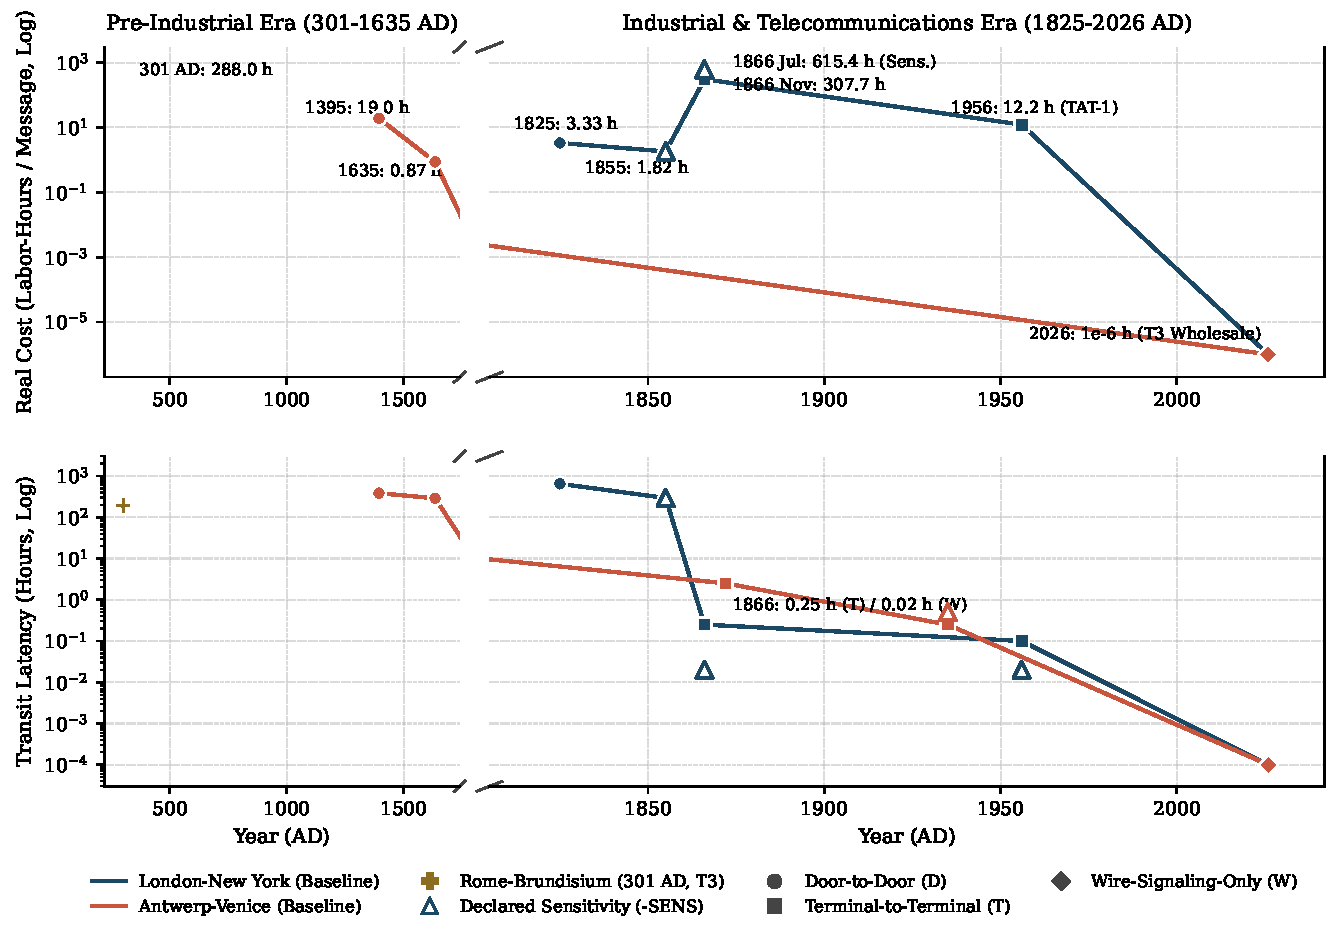
\includegraphics[width=0.98\textwidth]{figure1_macro_spine.pdf}
\caption{Four Millennia of Real Communication Costs and Transit Latency by Corridor, 301\,AD--2026\,AD. \textit{Notes:} Top panels plot real communication cost per standardized message (log scale); bottom panels plot physical transit latency (log scale). Solid lines connect chronological baseline observations within each corridor; hollow triangles denote declared sensitivity specifications ($250$-word limit at $1855$; July $1866$ $\gbp 20$ rate and $17\,\text{wpm}$ wire signaling); open circles with dotted stems denote estimated door-to-door bounds for terminal-to-terminal observations.}
\label{fig:macro_spine}
\end{figure}

Comparing these optical backbone figures directly with historical postal and telegraph rates, however, introduces an accounting boundary mismatch. Historical postal and telegraph tariffs measure retail transaction prices paid at the counter for an individual message, whereas $2026$ fiber lease rates measure bulk backbone capacity. Conversely, anchoring the $2026$ endpoint with consumer fixed-broadband subscriptions---which average $\gbp 37.50/\text{month}$ (range $\gbp 30.00$--$\gbp 45.00$) in the United Kingdom \citep{Ofcom2026} and $\$50.00/\text{month}$ (range $\$40.00$--$\$60.00$) in the United States \citep{FCC2026}---conflates fixed local-loop access, customer equipment, and billing overhead with the marginal cost of traversing distance (Table~\ref{tab:modern_boundary}). Separating wholesale backbone transit from retail last-mile access keeps the boundary definition consistent across the full four-millennium series.

\begin{table}[H]
\centering
\footnotesize
\begin{tabularx}{\textwidth}{@{}llccX@{}}
\toprule
\textbf{Scope Class} & \textbf{2026 Communication Benchmark} & \textbf{Baseline} & \textbf{Bounds} & \textbf{Unit / Tier / Source} \\
\midrule
Wholesale Backbone & European IP Transit (\texttt{DWDM}) & $2.00$ & $1.50$--$2.50$ & $€$/Mbps/mo (\texttt{T3}, \citealt{TeleGeography2026}) \\
Wholesale Backbone & Transatlantic Subsea Fiber & $7.80$ & $6.00$--$9.50$ & $\$$/Gbps/mo (\texttt{T3}, \citealt{SubTelForum2026}) \\
Retail Access & UK Fixed Broadband Subscription & $37.50$ & $30.00$--$45.00$ & $\gbp$/month (\texttt{T1}, \citealt{Ofcom2026}) \\
Retail Access & US Fixed Broadband Subscription & $50.00$ & $40.00$--$60.00$ & $\$$/month (\texttt{T1}, \citealt{FCC2026}) \\
\bottomrule
\end{tabularx}
\caption{2026 Modern Communication Scope Comparison: Wholesale Backbone vs.\ Retail Broadband}
\label{tab:modern_boundary}
\end{table}

\section{Conclusion}
\label{sec:conclusion}

Standardizing four millennia of communication tariffs by local wages, message word counts, and operational delivery boundaries shows that real messaging costs and physical transmission speeds followed distinct historical paths. Between $1395$ and $1855$, commercial postal networks reduced real messaging costs by more than two orders of magnitude while remaining bound to overland and maritime transport speeds. The $1866$ transatlantic submarine cable inverted that pattern, cutting transit time to minutes while raising real message costs $169$-fold ($3,381$-fold per word) and rationing early cable capacity to high-value financial and commodity arbitrageurs. Broadly affordable high-speed communication emerged only after competitive entry eroded cable cartels in the $1880\text{s}$ and twentieth-century multiplexing expanded channel capacity. All underlying datasets, archival shelfmark registers, and verification scripts (\path{scripts/audit_replication_package.py}) are archived at \url{https://github.com/rbastiaanssen-tech/cliometric-portal}.

\appendix

\section{Archival Evidence Taxonomy and Custodial Shelfmark Ledger}
\label{app:archival_ledger}

Every observation in our dataset is scored independently for tariff pricing (\textit{Tariff Tier}) and payload or throughput standardization (\textit{Capacity Tier}):
\begin{enumerate}
    \item \textbf{Tier 1 (\texttt{T1} --- Authenticated Primary):} Transcribed directly from contemporary statutory enactments, bilateral postal conventions, official gazettes, or primary corporate tariff schedules.
    \item \textbf{Tier 2 (\texttt{T2} --- Corroborated Secondary):} Established from peer-reviewed postal and economic historiography where physical folio scans from custodial archives remain queued for remote digitization.
    \item \textbf{Tier 3 (\texttt{T3} --- Parameterized Calibration):} Stylized institutional or engineering baselines where open-access commercial tariffs did not exist (Roman \textit{cursus publicus} shadow proxy and Tang \textit{Yizhan} relays) or where $2026$ marginal costs reflect wholesale backbone capacity allocations.
\end{enumerate}

Custodial shelfmarks queued for remote folio verification are logged in the replication repository: K\"ultepe cuneiform editions (\textit{BIN} 4 124, \textit{TPAK} 1 38); Tang statutory compendia (\textit{Yizhan tiaoli}); Archivio di Stato di Prato (\textit{Datini, buste 600--605}); F\"urst Thurn und Taxis Archiv (\textit{Postakten 1284}); The Postal Museum (\texttt{POST 43/112} ff.\ 84--88; \texttt{POST 101/184}); Archives Nationales (\texttt{F/90/21276}); BT Archives (\texttt{Ref:\ TGP}); PK Porthcurno (\texttt{BL C.132.h.27}); IET Archives (\texttt{UK0108 SC MSS 008}); and \citet{Scholliers1995} Belgian industrial wage series.

\section{Quote-Age Risk Derivations and Volatility Scaling ($H^*$)}
\label{app:quote_age}

Evaluating Equation~\eqref{eq:breakeven_h} across the $1866$ transatlantic transition reconciles our baseline break-even parameter $H^*_0$ with the sensitivity bounds in \texttt{public/data/sensitivity\_parameters.csv}:
\begin{itemize}
    \item \textbf{Baseline Break-Even Derivation ($H^*_0 = 2.515\,\text{LH/h}$):} Pairing the July $1866$ opening cable tariff ($C_{\text{telegraph}} = 615.38\,\text{LH}$, $L_{\text{telegraph}} = 0.25\,\text{h}$) against the contemporary $1866$ pre-cable steamship mean crossing of $10.18\,\text{days}$ ($L_{\text{packet, 1866}} = 244.20\,\text{h}$; \citealt{Steinwender2018}) and $C_{\text{packet}} = 1.82\,\text{LH}$ yields:
    \begin{equation}
    H^*_0 = \frac{615.38 - 1.82}{244.20 - 0.25} = \mathbf{2.515\,\text{labor-hours per hour of quote age}}.
    \end{equation}
    \item \textbf{Table~\ref{tab:master_benchmarks} 1855-Lag Comparisons:} Substituting Table~\ref{tab:master_benchmarks}'s $1855$ steam-packet mean crossing ($L_{\text{packet, 1855}} = 292.80\,\text{h}$) yields $H^*_{\text{1855, Jul}} = \frac{615.38 - 1.82}{292.80 - 0.25} = \mathbf{2.097\,\text{LH/h}}$ at the July tariff and $H^*_{\text{1855, Nov}} = \frac{307.69 - 1.82}{292.80 - 0.25} = \mathbf{1.046\,\text{LH/h}}$ at the November $\gbp 10$ tariff (comparing a 20-word cablegram against a 400-word letter; normalizing per 100 words gives $5.257\,\text{LH/h}$).
    \item \textbf{Steinwender (2018) Volatility Scaling:} Scaling $H^*_0 = 2.515$ across \citet{Steinwender2018}'s Table~3 log-variance lag elasticity range $\beta \in [0.13, 0.20]$ around $\beta_0 = 0.17\,\text{log points/day}$ ($\text{SE} = 0.08$) yields sensitivity bounds of:
    \begin{equation}
    H^*_{\text{low}} = 2.515 \times \frac{0.13}{0.17} = \mathbf{1.923\,\text{LH/h}}, \qquad
    H^*_{\text{high}} = 2.515 \times \frac{0.20}{0.17} = \mathbf{2.959\,\text{LH/h}}.
    \end{equation}
    Scaling $H^*_0$ to the post-cable standard deviation regime (\citealt{Steinwender2018}, Table~1: $93\%$ variance drop, $\sigma_{\text{post}} / \sigma_{\text{pre}} = \sqrt{0.07} = 0.265$) yields:
    \begin{equation}
    H^*_{\mathrm{SD\text{-}post}} = 2.515 \times 0.265 = \mathbf{0.666\,\text{LH/h}}.
    \end{equation}
\end{itemize}

\begin{thebibliography}{99}
\bibitem[Allen(2001)]{Allen2001} Allen, Robert C. 2001. ``The Great Divergence in European Wages and Prices from the Middle Ages to the First World War.'' \textit{Explorations in Economic History} 38(4): 411--447.
\bibitem[Allen(2007)]{Allen2007} Allen, Robert C. 2007. ``How Prosperous Were the Romans? Evidence from Diocletian's Price Edict (301 AD).'' Oxford Dept.\ of Economics Discussion Paper No.\ 363.
\bibitem[Arnell(1980)]{Arnell1980} Arnell, J. C. 1980. \textit{Steam and the North Atlantic Mails}. Toronto: Unitrade Press.
\bibitem[Behringer(1990)]{Behringer1990} Behringer, Wolfgang. 1990. \textit{Thurn und Taxis}. Munich: Piper.
\bibitem[Bogart(2005)]{Bogart2005} Bogart, Dan. 2005. ``Turnpike Trusts and the Transportation Revolution in 18th Century England.'' \textit{Explorations in Economic History} 42(4): 479--508.
\bibitem[Bowley(1900)]{Bowley1900} Bowley, Arthur L. 1900. \textit{Wages in the United Kingdom in the Nineteenth Century}. Cambridge: Cambridge University Press.
\bibitem[Bright(1866)]{Bright1866} Bright, Charles Tilston. 1866. ``The Atlantic Telegraph.'' \textit{Proceedings of the Institution of Civil Engineers} 25: 1--35.
\bibitem[Bright(1898)]{Bright1898} Bright, Charles. 1898. \textit{Submarine Telegraphs}. London: Crosby Lockwood.
\bibitem[British Parliamentary Papers(1849)]{BPP1849} British Parliamentary Papers. 1849. \textit{Convention between Her Majesty and the United States of America, for the Improvement of the Communication by Post}, Command Paper [1012]. London: HMSO.
\bibitem[British Parliamentary Papers(1855)]{BPP1855} British Parliamentary Papers. 1855. \textit{Mail Packet Returns: North American Mail Steamers}. London: HMSO.
\bibitem[Chandler(1977)]{Chandler1977} Chandler, Alfred D., Jr. 1977. \textit{The Visible Hand}. Cambridge, MA: Harvard University Press.
\bibitem[Dallmeier(1977)]{Dallmeier1977} Dallmeier, Martin. 1977. \textit{Quellen zur Geschichte des europ\"aischen Postwesens 1501--1806}. Kallm\"unz: Lassleben.
\bibitem[Dercksen(2004)]{Dercksen2004} Dercksen, Jan Gerrit. 2004. \textit{Old Assyrian Institutions}. Leiden: NINO.
\bibitem[Federal Communications Commission(2026)]{FCC2026} Federal Communications Commission (FCC). 2026. \textit{2026 Urban Rate Survey: Fixed Broadband Benchmark}. Washington, DC: FCC.
\bibitem[Frangioni(1994)]{Frangioni1994} Frangioni, Luciana. 1994. \textit{Organizzazione e costi del servizio postale alla fine del Trecento}. Prato: Istituto Datini.
\bibitem[Harley(1988)]{Harley1988} Harley, C. Knick. 1988. ``Ocean Freight Rates and Productivity, 1740--1913.'' \textit{Journal of Economic History} 48(4): 851--876.
\bibitem[Innis(1950)]{Innis1950} Innis, Harold A. 1950. \textit{Empire and Communications}. Oxford: Clarendon Press.
\bibitem[International Telegraph Union(1872)]{ITU1872} International Telegraph Union (ITU). 1872. \textit{Documents de la Conf\'erence T\'el\'egraphique Internationale de Rome}. Berne: Bureau International des Administrations T\'el\'egraphiques.
\bibitem[Joyce(1893)]{Joyce1893} Joyce, Herbert. 1893. \textit{The History of the Post Office}. London: Richard Bentley.
\bibitem[Kolb(2000)]{Kolb2000} Kolb, Anne. 2000. \textit{Transport und Nachrichtentransfer im R\"omischen Reich}. Berlin: Akademie Verlag.
\bibitem[Larsen(1976)]{Larsen1976} Larsen, Mogens Trolle. 1976. \textit{The Old Assyrian City-State and Its Colonies}. Copenhagen: Akademisk Forlag.
\bibitem[Malanima(2007)]{Malanima2007} Malanima, Paolo. 2007. ``Wages, Productivity and Working Time in Italy, 1300--1913.'' \textit{Journal of European Economic History} 36(1): 127--171.
\bibitem[Melis(1962)]{Melis1962} Melis, Federigo. 1962. \textit{Aspetti della vita economica medievale}. Siena: Monte dei Paschi.
\bibitem[Ministry of Labour(1956)]{MinLabour1956} Ministry of Labour and National Service. 1956. ``Earnings and Hours in October 1956.'' \textit{Ministry of Labour Gazette} 64(10): 361--368.
\bibitem[Nordhaus(1996)]{Nordhaus1996} Nordhaus, William D. 1996. ``Do Real-Output and Real-Wage Measures Capture Reality?'' In \textit{The Economics of New Goods}, 29--66. Chicago: University of Chicago Press.
\bibitem[North(1958)]{North1958} North, Douglass C. 1958. ``Ocean Freight Rates and Economic Development, 1750--1913.'' \textit{Journal of Economic History} 18(4): 537--555.
\bibitem[Ofcom(2026)]{Ofcom2026} Office of Communications (Ofcom). 2026. \textit{Pricing Trends for Communications Services in the UK (2026)}. London: Ofcom.
\bibitem[Pred(1973)]{Pred1973} Pred, Allan R. 1973. \textit{Urban Growth and the Circulation of Information}. Cambridge, MA: Harvard University Press.
\bibitem[R\"ubsam(1889)]{Rubsam1889} R\"ubsam, Josef. 1889. \textit{Johann Baptista von Taxis}. Freiburg: Herder.
\bibitem[Scholliers(1995)]{Scholliers1995} Scholliers, Peter. 1995. ``A Century of Real Industrial Wages in Belgium, 1840--1939.'' In \textit{Labour's Reward}, edited by P.\ Scholliers and V.\ Zamagni, 106--137. Aldershot: Edward Elgar.
\bibitem[Steinwender(2018)]{Steinwender2018} Steinwender, Claudia. 2018. ``Real Effects of Information Frictions: When the States and the Kingdom Became United.'' \textit{American Economic Review} 108(3): 657--696.
\bibitem[Submarine Telecoms Forum(2026)]{SubTelForum2026} Submarine Telecoms Forum. 2026. \textit{Submarine Telecoms Industry Report, 14th Edition}. Sterling, VA: Submarine Telecoms Forum.
\bibitem[TeleGeography(2026)]{TeleGeography2026} TeleGeography. 2026. \textit{Global Internet Geography \& IP Transit Pricing Report (2026)}. Washington, DC: PriMetrica.
\bibitem[U.S.\ Bureau of the Census(1960)]{USCensus1960} U.S.\ Bureau of the Census. 1960. \textit{Historical Statistics of the United States, Colonial Times to 1957}. Washington, DC: GPO.
\bibitem[Van der Wee(1963)]{VanderWee1963} Van der Wee, Herman. 1963. \textit{The Growth of the Antwerp Market and the European Economy}. The Hague: Martinus Nijhoff.
\bibitem[Veenhof(2008)]{Veenhof2008} Veenhof, Klaas R. 2008. ``The Old Assyrian Period.'' In \textit{Mesopotamia: The Old Assyrian Period}, 13--264. Fribourg: Academic Press.
\bibitem[Webb(1888)]{Webb1888} Webb, Frederick Charles. 1888. ``Thirty-Six Years in the Telegraphic Service.'' \textit{The Electrician} 21: 42--44.
\bibitem[Yan(1969)]{Yan1969} Yan, Gengwang. 1969. \textit{Tangdai jiaotong tu kao}. Taipei: Academia Sinica.
\end{thebibliography}

\end{document}
